\subsection{MVC} 
MVC or Model-View-Controller\cite{aspmvc} is used to separate responsibility of an application into three parts, the model, the view, and the controller.
The pattern can be seen in \Cref{mvcdiagram}.

\begin{figure}[h]
\begin{center}
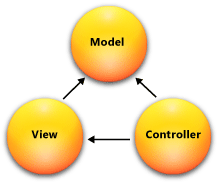
\includegraphics[width=\textwidth, trim={-4cm 11cm 5cm 1cm}]{mvc.pdf}
\caption{The MVC design pattern.}
\label{mvcdiagram}
\end{center}
\end{figure}

\paragraph{Model} contains the model of the application domain and takes care of fetching data from the underlying layers and making it available to the view and the controller.
In the case of our web service, the model is making resources available to the view.
\mikkel{Jeg synes at vi med den sidste linie siger at der ikke er forbindelse fra controller til model i vores web service.}
\mikkel{Generelt: Der er forskel på hvordan vi bruger paragraphs i rapporten - skal vi have ensrettet det?}

\paragraph{View} displays the model to the user.
In our case the view is the serialized resource representation, that the user obtains by performing requests against the API.
Per default, this is \texttt{text/xml}, however, by adding the \texttt{Accept} header, this can be set to \texttt{application/json} \cite[Section 14]{http_specification}.

\paragraph{Controller} handles the interaction with users.
Based on user input, the controller works on the model and selects what the view needs to be used for displaying the data.
\mikkel{''what the view needs to be used for displaying the data'' - jeg forstår ikke sætningen :/}

The routing to controllers is handled by the attributes \texttt{[RoutePrefix]} and \texttt{[Route]}.
In order to handle the different HTTP methods, controller methods are also annotated with an appropriate \texttt{[Http\{Method\}]} attribute (e.g. \texttt{[HttpGet]}) \cite{asp_routing}.
\mikkel{Jeg går ud fra at alle de ting der står i [ ] parenteser er attributes i C\#. Det synes jeg vi er nød til at præcisere.}
\mikkel{Jeg synes den ekstra information om routing adskiller sig meget fra den øvrige beskrivelse - er det ikke en uinteressant detalje?}